% CVPR 2024 Paper Template; see https://github.com/cvpr-org/author-kit

\documentclass[10pt,twocolumn,letterpaper]{article}
%%%%%%%%% PAPER TYPE  - PLEASE UPDATE FOR FINAL VERSION
\usepackage{cvpr}              % To produce the CAMERA-READY version
% \usepackage[review]{cvpr}      % To produce the REVIEW version
% \usepackage[pagenumbers]{cvpr} % To force page numbers, e.g. for an arXiv version

% Import additional packages in the preamble file, before hyperref
\setlength{\parskip}{0pt}
%
% --- inline annotations
%
\usepackage[dvipsnames]{xcolor}
\newcommand{\red}[1]{{\color{red}#1}}
\newcommand{\todo}[1]{{\color{red}#1}}
\newcommand{\TODO}[1]{\textbf{\color{red}[TODO: #1]}}
% --- disable by uncommenting  
% \renewcommand{\TODO}[1]{}
% \renewcommand{\todo}[1]{#1}



% It is strongly recommended to use hyperref, especially for the review version.
% hyperref with option pagebackref eases the reviewers' job.
% Please disable hyperref *only* if you encounter grave issues, 
% e.g. with the file validation for the camera-ready version.
%
% If you comment hyperref and then uncomment it, you should delete *.aux before re-running LaTeX.
% (Or just hit 'q' on the first LaTeX run, let it finish, and you should be clear).
\definecolor{cvprblue}{rgb}{0.21,0.49,0.74}
\usepackage[pagebackref,breaklinks,colorlinks,citecolor=cvprblue]{hyperref}


%%%%%%%%% PAPER ID  - PLEASE UPDATE
\def\paperID{*****} % *** Enter the Paper ID here
\def\confName{CVPR}
\def\confYear{2024}

%%%%%%%%% TITLE - PLEASE UPDATE
\title{DanceVision Proposal}

%%%%%%%%% AUTHORS - PLEASE UPDATE
\author{Anna Guo \qquad Jenna Jacob \qquad Katie Wang \qquad Natalie Leal Blanco\\
UT Austin: Computer Vision Course\\
% Institution1 address\\
{\tt\small annayuab@icloud.com}\\
% For a paper whose authors are all at the same institution,
% omit the following lines up until the closing ``}''.
% Additional authors and addresses can be added with ``\and'',
% just like the second author.
% To save space, use either the email address or home page, not both
\and
% Institution2\\
% First line of institution2 address\\
% {\tt\small secondauthor@i2.org}
}

\begin{document}
\maketitle
\begin{abstract}
The ABSTRACT is to be in fully justified italicized text, at the top of the left-hand column, below the author and affiliation information.
Use the word ``Abstract'' as the title, in 12-point Times, boldface type, centered relative to the column, initially capitalized.
The abstract is to be in 10-point, single-spaced type.
Leave two blank lines after the Abstract, then begin the main text.
Look at previous \confName abstracts to get a feel for style and length.
\end{abstract}    
\section{Introduction}
\label{sec:intro}

\indent Over 50 million Americans seek physical therapy every year, whether that be from 
musculoskeletal conditions, car accidents, or sports injuries. Evidently, there is a large
need for physical therapy. However, only 35% of PT patients actually adhere to their assigned 
plan. This is a significant problem since the majority of patients are not following 
through with their exercises and thus decrease the effectiveness of their therapy plan.
\\
\indent We aim to use Computer Vision to partition each exercise movement into more easily digestible chunks 
by creating a model that can learn (vectorize) each exercise movement from two given videos, an instructional 
one and a patient one, and compare the two. By developing a tool that provides feedback as a result of analyzing 
the two videos, which ideally should match perfectly, adhering to an exercise plan 
becomes much more feasible, enjoyable, and even motivating.

%-------------------------------------------------------------------------
\subsection{Existing Attempts}
\indent Several existing attempts have been made to tackle the challenge of improving patient adherence, 
each with its own approach and limitations. One such approach involves utilizing monitoring technology, 
such as pedometers, which have proved to be user-friendly. Though such monitoring technologies are 
able to monitor, or track, the patients' physical activity decently well, there was not much of an effect in terms 
of improving their adherence to their exercise plans. As a result, patients using such technologies still struggle with 
adhering to their exercise plans.
\\
\indent Another attempt that has been made is virtual and augmented reality treatment. Through this method, patients 
are able to put on their VR headsets and transport into any environment they would like to complete their exercises in. 
The possibilities are endless: they could surround themselves in peaceful, serene nature, or they could 
opt for a more competitive gaming atmosphere. Physical therapists have found that this actually 
makes their treatment plans more appealing and thus improves their patient adherence rates. However, 
it is important to note that this is significantly more expensive. The cost associated with this 
method is typically too high for the majority of patients and thus makes this approach less practical.
\\
\indent Unlike the aforementioned methods, our proposed method is low-cost, accessible, and effective. 
Implementing the aspect of gamification allows for physical therapy to be fun yet productive. Patients become 
competitors, working hard to beat their previous scores. Additionally, our method could be expanded to offer 
further personalized feedback based on the analysis of the learner's own video and the given instructional video, 
ideally without the requirement for perfect lighting or camera angle conditions.

\subsection{Useful Techniques}
\indent Several computer vision techniques offer promising avenues for addressing the challenge of learning 
exercising movements from instructional videos by providing deeper insights into their dynamics and nuances. 
One such technique involves exploring 3D models instead of traditional 2D skeletonization
 methods to create more comprehensive representations of the exercise movements. Unlike 2D skeletonization, 
 which captures only the spatial coordinates of key body joints in a single plane, 3D modeling 
 techniques can capture the full spatial extent of exericse movements, including depth information\cite{Alpher03}. This 
 allows for a more accurate and detailed representation of the individual's body and movements in 
 three-dimensional space, which is particularly valuable for capturing complex and multi-dimensional 
 exercise movements\cite{Authors14b}.
\\
\indent In addition to 3D modeling, other computer vision techniques such as action recognition, pose 
estimation, trajectory analysis, and video segmentation and tracking can provide valuable insights 
into the dynamics of exercise movements. Action recognition algorithms can automatically identify and 
classify different gestures and even exercise sequences, allowing for automated analysis of exercise 
patterns and styles. Pose estimation techniques can accurately estimate the skeletal poses of 
people from video frames, providing a structural representation of their movements that can be 
used for further analysis and interpretation.
\\
\indent Trajectory analysis techniques can track the trajectories of specific body parts or exercise movements 
over time, allowing for the analysis of exercise movement patterns, velocities, and accelerations\cite{Alpher02}. This 
provides valuable insights into the dynamic aspects of these exercises, 
helping learners to better understand the timing and pacing of the movements. Video segmentation and 
tracking methods also serve to segment the videos into individual sequences or movements, allowing for more 
focused analysis and comparison of specific elements.
\\
\indent By leveraging these advanced computer vision techniques, learners can gain a deeper understanding 
of the dynamics and nuances of exercise movements, facilitating more effective learning experiences. 
These techniques can help learners to break down complex movements into smaller, more 
manageable components, identify areas for improvement, and refine their technique with greater 
precision and accuracy. Overall, the integration of computer vision into physical therapy has the 
potential to revolutionize the way patients approach their recovery plan, making it more accessible, engaging, 
and effective for patients of all levels.

\subsection{Challenges}
\indent Several challenges arise from attempting this project. One is the quality of input data, which 
encompasses various factors such as lighting, angles, occlusions, frame rates, and blurring. These 
factors can significantly impact the accuracy of movement analysis, as they can obscure or distort 
key visual information needed for understanding exercise movements. Addressing these challenges may 
require the development of robust computer vision algorithms capable of handling noisy or low-quality 
video data, as well as techniques for preprocessing and enhancing the visual information to improve 
analysis accuracy.
\\
\indent Moreover, handling interactions between multiple persons in an input video presents additional 
complexities in accurately capturing and representing exercise movements. In some videos, 
there may be two individuals present that interact with each other in complex ways. It is not uncommon for  
one to assist the other in certain movements, for example, by helping lift up or stretch their legs. 
Capturing these interactions and accurately representing them in the analysis poses challenges for 
computer vision algorithms, as they must be able to differentiate between individuals 
and track their movements independently while also accounting for their interactions with others. 
Addressing this challenge may require the development of advanced tracking and segmentation techniques 
capable of accurately identifying and tracking multiple persons in a dynamic environment.
\\
\indent Overall, addressing these challenges requires a multidisciplinary approach that combines expertise 
in computer vision, exercise analysis, and human-computer interaction. By developing robust algorithms, 
incorporating domain-specific knowledge, and leveraging advanced techniques for handling complex 
visual data, it is possible to create a tool that effectively supports learning exercises from  
videos using computer vision. However, continued research and development efforts are needed to 
overcome these challenges and realize the full potential of computer vision technology in the 
field of physical therapy.

\subsection{Technical Gap}
\indent The primary aim of this project is to reduce the technical gap between physical therapy videos and 
effective recovery plans. By enabling the correspondence between individuals with different body proportions 
captured from various angles, this tool seeks to enhance the accessibility and inclusivity of these exercises plans. 
This interdisciplinary endeavor involves collaboration between experts in physical therapy, biomechanics, and computer 
vision, with computer vision providing quantitative analysis capabilities to enhance the understanding and 
teaching of exercise movements.
\\
\indent In conclusion, developing a tool for learning exercises from physical therapy videos using computer vision holds 
great potential for revolutionizing physical therapy plans and making them more accessible and doable to a wider 
audience. By leveraging advanced computer vision techniques and interdisciplinary collaboration, 
this project aims to bridge the gap between physical therapy videos and effective recovery plans, 
ultimately empowering individuals to learn and appreciate physical therapy in new and innovative ways.

% \subsection{Paper length}
% Papers, excluding the references section, must be no longer than eight pages in length.
% The references section will not be included in the page count, and there is no limit on the length of the references section.
% For example, a paper of eight pages with two pages of references would have a total length of 10 pages.
% {\bf There will be no extra page charges for \confName\ \confYear.}

% Overlength papers will simply not be reviewed.
% This includes papers where the margins and formatting are deemed to have been significantly altered from those laid down by this style guide.
% Note that this \LaTeX\ guide already sets figure captions and references in a smaller font.
% The reason such papers will not be reviewed is that there is no provision for supervised revisions of manuscripts.
% The reviewing process cannot determine the suitability of the paper for presentation in eight pages if it is reviewed in eleven.

% %-------------------------------------------------------------------------
% \subsection{The ruler}
% The \LaTeX\ style defines a printed ruler which should be present in the version submitted for review.
% The ruler is provided in order that reviewers may comment on particular lines in the paper without circumlocution.
% If you are preparing a document using a non-\LaTeX\ document preparation system, please arrange for an equivalent ruler to appear on the final output pages.
% The presence or absence of the ruler should not change the appearance of any other content on the page.
% The camera-ready copy should not contain a ruler.
% (\LaTeX\ users may use options of \texttt{cvpr.sty} to switch between different versions.)

% Reviewers:
% note that the ruler measurements do not align well with lines in the paper --- this turns out to be very difficult to do well when the paper contains many figures and equations, and, when done, looks ugly.
% Just use fractional references (\eg, this line is $087.5$), although in most cases one would expect that the approximate location will be adequate.


% \subsection{Paper ID}
% Make sure that the Paper ID from the submission system is visible in the version submitted for review (replacing the ``*****'' you see in this document).
% If you are using the \LaTeX\ template, \textbf{make sure to update paper ID in the appropriate place in the tex file}.


% \subsection{Mathematics}

% Please number all of your sections and displayed equations as in these examples:
% \begin{equation}
%   E = m\cdot c^2
%   \label{eq:important}
% \end{equation}
% and
% \begin{equation}
%   v = a\cdot t.
%   \label{eq:also-important}
% \end{equation}
% It is important for readers to be able to refer to any particular equation.
% Just because you did not refer to it in the text does not mean some future reader might not need to refer to it.
% It is cumbersome to have to use circumlocutions like ``the equation second from the top of page 3 column 1''.
% (Note that the ruler will not be present in the final copy, so is not an alternative to equation numbers).
% All authors will benefit from reading Mermin's description of how to write mathematics:
% \url{http://www.pamitc.org/documents/mermin.pdf}.

% \subsection{Blind review}

% Many authors misunderstand the concept of anonymizing for blind review.
% Blind review does not mean that one must remove citations to one's own work---in fact it is often impossible to review a paper unless the previous citations are known and available.

% Blind review means that you do not use the words ``my'' or ``our'' when citing previous work.
% That is all.
% (But see below for tech reports.)

% Saying ``this builds on the work of Lucy Smith [1]'' does not say that you are Lucy Smith;
% it says that you are building on her work.
% If you are Smith and Jones, do not say ``as we show in [7]'', say ``as Smith and Jones show in [7]'' and at the end of the paper, include reference 7 as you would any other cited work.

% An example of a bad paper just asking to be rejected:
% \begin{quote}
% \begin{center}
%     An analysis of the frobnicatable foo filter.
% \end{center}

%    In this paper we present a performance analysis of our previous paper [1], and show it to be inferior to all previously known methods.
%    Why the previous paper was accepted without this analysis is beyond me.

%    [1] Removed for blind review
% \end{quote}


% An example of an acceptable paper:
% \begin{quote}
% \begin{center}
%      An analysis of the frobnicatable foo filter.
% \end{center}

%    In this paper we present a performance analysis of the  paper of Smith \etal [1], and show it to be inferior to all previously known methods.
%    Why the previous paper was accepted without this analysis is beyond me.

%    [1] Smith, L and Jones, C. ``The frobnicatable foo filter, a fundamental contribution to human knowledge''. Nature 381(12), 1-213.
% \end{quote}

% If you are making a submission to another conference at the same time, which covers similar or overlapping material, you may need to refer to that submission in order to explain the differences, just as you would if you had previously published related work.
% In such cases, include the anonymized parallel submission~\cite{Authors14} as supplemental material and cite it as
% \begin{quote}
% [1] Authors. ``The frobnicatable foo filter'', F\&G 2014 Submission ID 324, Supplied as supplemental material {\tt fg324.pdf}.
% \end{quote}

% Finally, you may feel you need to tell the reader that more details can be found elsewhere, and refer them to a technical report.
% For conference submissions, the paper must stand on its own, and not {\em require} the reviewer to go to a tech report for further details.
% Thus, you may say in the body of the paper ``further details may be found in~\cite{Authors14b}''.
% Then submit the tech report as supplemental material.
% Again, you may not assume the reviewers will read this material.

% Sometimes your paper is about a problem which you tested using a tool that is widely known to be restricted to a single institution.
% For example, let's say it's 1969, you have solved a key problem on the Apollo lander, and you believe that the 1970 audience would like to hear about your
% solution.
% The work is a development of your celebrated 1968 paper entitled ``Zero-g frobnication: How being the only people in the world with access to the Apollo lander source code makes us a wow at parties'', by Zeus \etal.

% You can handle this paper like any other.
% Do not write ``We show how to improve our previous work [Anonymous, 1968].
% This time we tested the algorithm on a lunar lander [name of lander removed for blind review]''.
% That would be silly, and would immediately identify the authors.
% Instead write the following:
% \begin{quotation}
% \noindent
%    We describe a system for zero-g frobnication.
%    This system is new because it handles the following cases:
%    A, B.  Previous systems [Zeus et al. 1968] did not  handle case B properly.
%    Ours handles it by including a foo term in the bar integral.

%    ...

%    The proposed system was integrated with the Apollo lunar lander, and went all the way to the moon, don't you know.
%    It displayed the following behaviours, which show how well we solved cases A and B: ...
% \end{quotation}
% As you can see, the above text follows standard scientific convention, reads better than the first version, and does not explicitly name you as the authors.
% A reviewer might think it likely that the new paper was written by Zeus \etal, but cannot make any decision based on that guess.
% He or she would have to be sure that no other authors could have been contracted to solve problem B.
% \medskip

% \noindent
% FAQ\medskip\\
% {\bf Q:} Are acknowledgements OK?\\
% {\bf A:} No.  Leave them for the final copy.\medskip\\
% {\bf Q:} How do I cite my results reported in open challenges?
% {\bf A:} To conform with the double-blind review policy, you can report results of other challenge participants together with your results in your paper.
% For your results, however, you should not identify yourself and should not mention your participation in the challenge.
% Instead present your results referring to the method proposed in your paper and draw conclusions based on the experimental comparison to other results.\medskip\\

% \begin{figure}[t]
%   \centering
%   \fbox{\rule{0pt}{2in} \rule{0.9\linewidth}{0pt}}
%    %\includegraphics[width=0.8\linewidth]{egfigure.eps}

%    \caption{Example of caption.
%    It is set in Roman so that mathematics (always set in Roman: $B \sin A = A \sin B$) may be included without an ugly clash.}
%    \label{fig:onecol}
% \end{figure}

% \subsection{Miscellaneous}

% \noindent
% Compare the following:\\
% \begin{tabular}{ll}
%  \verb'$conf_a$' &  $conf_a$ \\
%  \verb'$\mathit{conf}_a$' & $\mathit{conf}_a$
% \end{tabular}\\
% See The \TeX book, p165.

% The space after \eg, meaning ``for example'', should not be a sentence-ending space.
% So \eg is correct, {\em e.g.} is not.
% The provided \verb'\eg' macro takes care of this.

% When citing a multi-author paper, you may save space by using ``et alia'', shortened to ``\etal'' (not ``{\em et.\ al.}'' as ``{\em et}'' is a complete word).
% If you use the \verb'\etal' macro provided, then you need not worry about double periods when used at the end of a sentence as in Alpher \etal.
% However, use it only when there are three or more authors.
% Thus, the following is correct:
%    ``Frobnication has been trendy lately.
%    It was introduced by Alpher~\cite{Alpher02}, and subsequently developed by
%    Alpher and Fotheringham-Smythe~\cite{Alpher03}, and Alpher \etal~\cite{Alpher04}.''

% This is incorrect: ``... subsequently developed by Alpher \etal~\cite{Alpher03} ...'' because reference~\cite{Alpher03} has just two authors.

% \begin{figure*}
%   \centering
%   \begin{subfigure}{0.68\linewidth}
%     \fbox{\rule{0pt}{2in} \rule{.9\linewidth}{0pt}}
%     \caption{An example of a subfigure.}
%     \label{fig:short-a}
%   \end{subfigure}
%   \hfill
%   \begin{subfigure}{0.28\linewidth}
%     \fbox{\rule{0pt}{2in} \rule{.9\linewidth}{0pt}}
%     \caption{Another example of a subfigure.}
%     \label{fig:short-b}
%   \end{subfigure}
%   \caption{Example of a short caption, which should be centered.}
%   \label{fig:short}
% \end{figure*}

\section{Pose Estimation Models}
\label{sec:pose}

The first step in developing this project was to define the parameters and requirements in order to choose models and algorithms that satisfy our expectations.
The first model that will be implemented on our project is a Pose Estimation Model. The requirements we defined were: limit GPU usage, multiple persons detection, 
and output in the form of JSON files, in order to be transferable and readible for the subsequent sections of our project.  We also set a high priority on accuracy,
due to the requirements for the other portions of our project\cite{Alpher08}. The following section will highlight our research, testing, and challenges, as well as the 
factors that influenced our decision-making process.

%-------------------------------------------------------------------------
\subsection{Model Choices}
 
In order for our project to work as intended, we needed to make sure we started by using the optimal tools for data collection. Our project was in need of a pose estimation model, and some options that we considered were OpenPose, MediaPipe, and MoveNet.
\\
\begin{enumerate}
    \item MediaPipe: MediaPipe is a Framework with many applications that have been widely used by Google for numerous products and services\cite{Authors14f}. For this project specifically, MediaPipe would aid specifically in pose detection and video processing using OpenCV. 
    Unfortunately, this is limited to single-person analysis, and we wanted to account for the possibility of expanding our project to process videos with multiple people.
    \\
    \item MoveNet: MoveNet is another pose estimation model that we considered. Developed by Google, it utilizes deep learning techniques, and is an improved version of the previous generation PoseNet model (released in 2017)\cite{Authors14a}. Though this processed our videos 
    quickly, it did not have the desired accuracy for the video inputs (key points tended to be in the general region of the desired body parts but didn’t always overlap fully, which led to doubts on its ability to capture the fine granularity we wanted for 
    detailed dance movements).
    \\
    \item OpenPose: OpenPose is yet another software for pose estimation, which has proved to work well when evaluating multiple persons, even for more crowded scenes. It uses a bottom-up approach to produce higher quality results, though at a higher 
    computational cost compared to MediaPipe and MoveNet\cite{Alpher07}. Additionally, it outputs JSON files, one per video frame, containing data for keypoints (e.g., left knee, right knee, etc.) that were easier to process. \\
\end{enumerate}

Because of its high accuracy and usable output, OpenPose was selected for this project over MediaPipe and MoveNet.

\subsection{Challenges with OpenPose}

Initially, OpenPose appeared to require more significant computational resources than were readily available to us (RAM and GPU), but we were able to run the model 
successfully after closing other running programs on our computers and using the CPU-version of OpenPose. 
\\
\indent As we became more familiar with OpenPose, we began testing the effects of different parameters. For instance, we learned that lowering the resolution of a video 
resulted in a significantly faster processing time. However, this also  caused decreased accuracy in the pose estimation. Thus, after several rounds of testing, 
we decided against reducing the resolution in our input videos since our project performance doesn’t depend on low latency, but does benefit from higher accuracy.



% \subsection{Paper length}
% Papers, excluding the references section, must be no longer than eight pages in length.
% The references section will not be included in the page count, and there is no limit on the length of the references section.
% For example, a paper of eight pages with two pages of references would have a total length of 10 pages.
% {\bf There will be no extra page charges for \confName\ \confYear.}

% Overlength papers will simply not be reviewed.
% This includes papers where the margins and formatting are deemed to have been significantly altered from those laid down by this style guide.
% Note that this \LaTeX\ guide already sets figure captions and references in a smaller font.
% The reason such papers will not be reviewed is that there is no provision for supervised revisions of manuscripts.
% The reviewing process cannot determine the suitability of the paper for presentation in eight pages if it is reviewed in eleven.

% %-------------------------------------------------------------------------
% \subsection{The ruler}
% The \LaTeX\ style defines a printed ruler which should be present in the version submitted for review.
% The ruler is provided in order that reviewers may comment on particular lines in the paper without circumlocution.
% If you are preparing a document using a non-\LaTeX\ document preparation system, please arrange for an equivalent ruler to appear on the final output pages.
% The presence or absence of the ruler should not change the appearance of any other content on the page.
% The camera-ready copy should not contain a ruler.
% (\LaTeX\ users may use options of \texttt{cvpr.sty} to switch between different versions.)

% Reviewers:
% note that the ruler measurements do not align well with lines in the paper --- this turns out to be very difficult to do well when the paper contains many figures and equations, and, when done, looks ugly.
% Just use fractional references (\eg, this line is $087.5$), although in most cases one would expect that the approximate location will be adequate.


% \subsection{Paper ID}
% Make sure that the Paper ID from the submission system is visible in the version submitted for review (replacing the ``*****'' you see in this document).
% If you are using the \LaTeX\ template, \textbf{make sure to update paper ID in the appropriate place in the tex file}.


% \subsection{Mathematics}

% Please number all of your sections and displayed equations as in these examples:
% \begin{equation}
%   E = m\cdot c^2
%   \label{eq:important}
% \end{equation}
% and
% \begin{equation}
%   v = a\cdot t.
%   \label{eq:also-important}
% \end{equation}
% It is important for readers to be able to refer to any particular equation.
% Just because you did not refer to it in the text does not mean some future reader might not need to refer to it.
% It is cumbersome to have to use circumlocutions like ``the equation second from the top of page 3 column 1''.
% (Note that the ruler will not be present in the final copy, so is not an alternative to equation numbers).
% All authors will benefit from reading Mermin's description of how to write mathematics:
% \url{http://www.pamitc.org/documents/mermin.pdf}.

% \subsection{Blind review}

% Many authors misunderstand the concept of anonymizing for blind review.
% Blind review does not mean that one must remove citations to one's own work---in fact it is often impossible to review a paper unless the previous citations are known and available.

% Blind review means that you do not use the words ``my'' or ``our'' when citing previous work.
% That is all.
% (But see below for tech reports.)

% Saying ``this builds on the work of Lucy Smith [1]'' does not say that you are Lucy Smith;
% it says that you are building on her work.
% If you are Smith and Jones, do not say ``as we show in [7]'', say ``as Smith and Jones show in [7]'' and at the end of the paper, include reference 7 as you would any other cited work.

% An example of a bad paper just asking to be rejected:
% \begin{quote}
% \begin{center}
%     An analysis of the frobnicatable foo filter.
% \end{center}

%    In this paper we present a performance analysis of our previous paper [1], and show it to be inferior to all previously known methods.
%    Why the previous paper was accepted without this analysis is beyond me.

%    [1] Removed for blind review
% \end{quote}


% An example of an acceptable paper:
% \begin{quote}
% \begin{center}
%      An analysis of the frobnicatable foo filter.
% \end{center}

%    In this paper we present a performance analysis of the  paper of Smith \etal [1], and show it to be inferior to all previously known methods.
%    Why the previous paper was accepted without this analysis is beyond me.

%    [1] Smith, L and Jones, C. ``The frobnicatable foo filter, a fundamental contribution to human knowledge''. Nature 381(12), 1-213.
% \end{quote}

% If you are making a submission to another conference at the same time, which covers similar or overlapping material, you may need to refer to that submission in order to explain the differences, just as you would if you had previously published related work.
% In such cases, include the anonymized parallel submission~\cite{Authors14} as supplemental material and cite it as
% \begin{quote}
% [1] Authors. ``The frobnicatable foo filter'', F\&G 2014 Submission ID 324, Supplied as supplemental material {\tt fg324.pdf}.
% \end{quote}

% Finally, you may feel you need to tell the reader that more details can be found elsewhere, and refer them to a technical report.
% For conference submissions, the paper must stand on its own, and not {\em require} the reviewer to go to a tech report for further details.
% Thus, you may say in the body of the paper ``further details may be found in~\cite{Authors14b}''.
% Then submit the tech report as supplemental material.
% Again, you may not assume the reviewers will read this material.

% Sometimes your paper is about a problem which you tested using a tool that is widely known to be restricted to a single institution.
% For example, let's say it's 1969, you have solved a key problem on the Apollo lander, and you believe that the 1970 audience would like to hear about your
% solution.
% The work is a development of your celebrated 1968 paper entitled ``Zero-g frobnication: How being the only people in the world with access to the Apollo lander source code makes us a wow at parties'', by Zeus \etal.

% You can handle this paper like any other.
% Do not write ``We show how to improve our previous work [Anonymous, 1968].
% This time we tested the algorithm on a lunar lander [name of lander removed for blind review]''.
% That would be silly, and would immediately identify the authors.
% Instead write the following:
% \begin{quotation}
% \noindent
%    We describe a system for zero-g frobnication.
%    This system is new because it handles the following cases:
%    A, B.  Previous systems [Zeus et al. 1968] did not  handle case B properly.
%    Ours handles it by including a foo term in the bar integral.

%    ...

%    The proposed system was integrated with the Apollo lunar lander, and went all the way to the moon, don't you know.
%    It displayed the following behaviours, which show how well we solved cases A and B: ...
% \end{quotation}
% As you can see, the above text follows standard scientific convention, reads better than the first version, and does not explicitly name you as the authors.
% A reviewer might think it likely that the new paper was written by Zeus \etal, but cannot make any decision based on that guess.
% He or she would have to be sure that no other authors could have been contracted to solve problem B.
% \medskip

% \noindent
% FAQ\medskip\\
% {\bf Q:} Are acknowledgements OK?\\
% {\bf A:} No.  Leave them for the final copy.\medskip\\
% {\bf Q:} How do I cite my results reported in open challenges?
% {\bf A:} To conform with the double-blind review policy, you can report results of other challenge participants together with your results in your paper.
% For your results, however, you should not identify yourself and should not mention your participation in the challenge.
% Instead present your results referring to the method proposed in your paper and draw conclusions based on the experimental comparison to other results.\medskip\\

% \begin{figure}[t]
%   \centering
%   \fbox{\rule{0pt}{2in} \rule{0.9\linewidth}{0pt}}
%    %\includegraphics[width=0.8\linewidth]{egfigure.eps}

%    \caption{Example of caption.
%    It is set in Roman so that mathematics (always set in Roman: $B \sin A = A \sin B$) may be included without an ugly clash.}
%    \label{fig:onecol}
% \end{figure}

% \subsection{Miscellaneous}

% \noindent
% Compare the following:\\
% \begin{tabular}{ll}
%  \verb'$conf_a$' &  $conf_a$ \\
%  \verb'$\mathit{conf}_a$' & $\mathit{conf}_a$
% \end{tabular}\\
% See The \TeX book, p165.

% The space after \eg, meaning ``for example'', should not be a sentence-ending space.
% So \eg is correct, {\em e.g.} is not.
% The provided \verb'\eg' macro takes care of this.

% When citing a multi-author paper, you may save space by using ``et alia'', shortened to ``\etal'' (not ``{\em et.\ al.}'' as ``{\em et}'' is a complete word).
% If you use the \verb'\etal' macro provided, then you need not worry about double periods when used at the end of a sentence as in Alpher \etal.
% However, use it only when there are three or more authors.
% Thus, the following is correct:
%    ``Frobnication has been trendy lately.
%    It was introduced by Alpher~\cite{Alpher02}, and subsequently developed by
%    Alpher and Fotheringham-Smythe~\cite{Alpher03}, and Alpher \etal~\cite{Alpher04}.''

% This is incorrect: ``... subsequently developed by Alpher \etal~\cite{Alpher03} ...'' because reference~\cite{Alpher03} has just two authors.

% \begin{figure*}
%   \centering
%   \begin{subfigure}{0.68\linewidth}
%     \fbox{\rule{0pt}{2in} \rule{.9\linewidth}{0pt}}
%     \caption{An example of a subfigure.}
%     \label{fig:short-a}
%   \end{subfigure}
%   \hfill
%   \begin{subfigure}{0.28\linewidth}
%     \fbox{\rule{0pt}{2in} \rule{.9\linewidth}{0pt}}
%     \caption{Another example of a subfigure.}
%     \label{fig:short-b}
%   \end{subfigure}
%   \caption{Example of a short caption, which should be centered.}
%   \label{fig:short}
% \end{figure*}

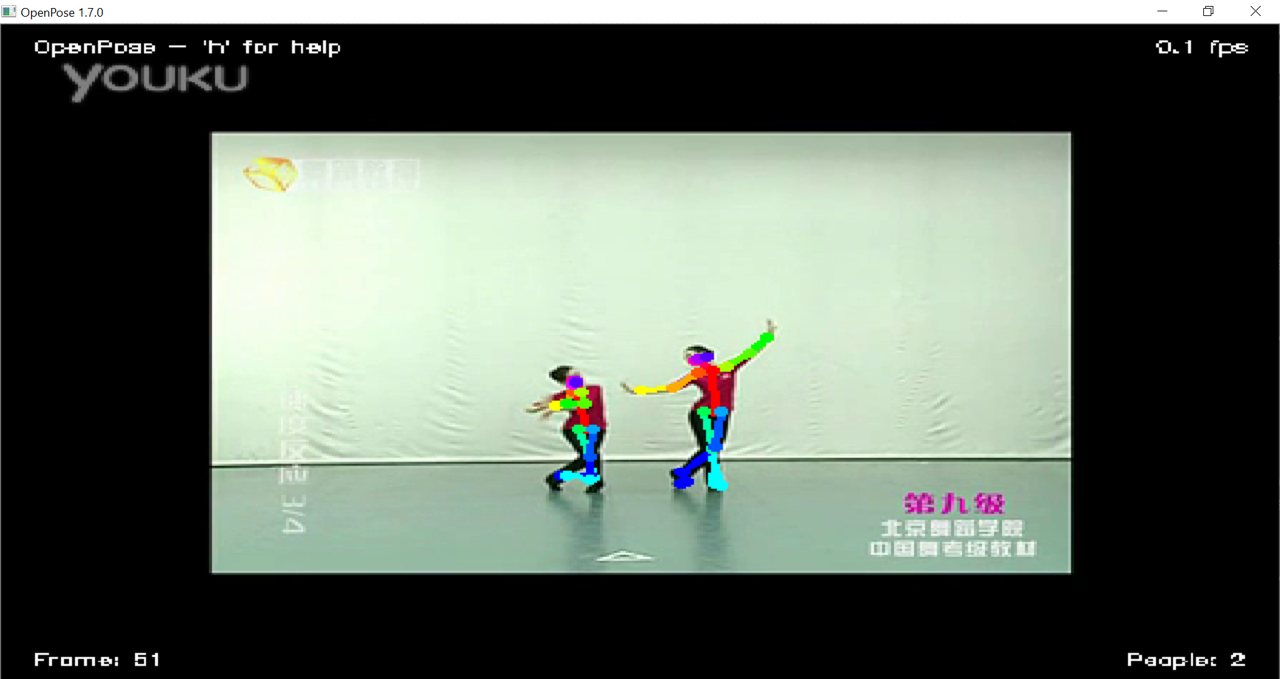
\includegraphics[width=\columnwidth]{sec/openpose_demo}
\textit{Figure 1. OpenPose in action: pose detection on a frame from an input video of two people. 
OpenPose accurately detects the key points on both people despite their slightly unorthodox body positions.}
\section{Algorithm to Prepare OpenPose outputs for Feature Extraction}
\label{sec:algorithm}

For a given video, OpenPose outputs a directory of json files, with one for each frame. Before passing these outputs to a second machine learning model, 
we want to write an algorithm that maps similar movements to the same values, regardless of camera angle or proximity of the person to the camera. 
(Due to the nature of OpenPose outputting x, y values for keypoints, we have already circumvented the issue of changes in illumination.)  Our algorithm aims to:
\\
\begin{enumerate}
    \item Remove absolute position by calculating the change in positions of key points between consecutive frames.
    \\
    \item Normalize position gradient using the maximum distance (in the 32 most recent frames) from right shoulder to right hip.
    \\
    \item Accommodate consistent elliptical motion by calculating angles at body joints.
\end{enumerate}

We choose to transition away from absolute positions to position gradients due to inspiration from SIFT’s usage of illumination gradients. Absolute positions 
could cause our model to unintentionally train on a dancer’s location in the camera view rather than their movements, whereas position gradient should make our 
model invariant to the dancer’s x, y-positions.
\\
\indent Similarly, by attempting to normalize the position gradients to the length of the dancer’s body part, we hope to make our model invariant to the dancer’s height 
and their distance from the camera (people in the foreground tend to appear taller than people in the background). We choose the right shoulder and right hip 
specifically because we believe the distance in between to represent a relatively rigid part of the body with a length correlated to a person’s height. Furthermore, 
we choose the longest length found to account for dance movements that may cause the shoulder and hip to be closer together than usual, while limiting the range to 
2 seconds (32 frames) so that we’re still sensitive to global changes (changes throughout the video) in z position (the distance between the dancer and camera center).
\\
\indent Finally, we want to pass in angles calculated from the keypoints. Firstly, this will likely aid the model in considering elliptical motions, which are prevalent in dances, 
as a continuous motion, as opposed to a single elliptical motion being calculated as multiple straight-line movements. Additionally, this encodes information about body parts 
relative to each other. For instance, moving one’s right hand downwards on the left side of one’s body could be differentiated from moving one’s right hand downwards on the right
 side of one’s body through the angle of the right elbow relative to the right shoulder.


% \subsection{Paper length}
% Papers, excluding the references section, must be no longer than eight pages in length.
% The references section will not be included in the page count, and there is no limit on the length of the references section.
% For example, a paper of eight pages with two pages of references would have a total length of 10 pages.
% {\bf There will be no extra page charges for \confName\ \confYear.}

% Overlength papers will simply not be reviewed.
% This includes papers where the margins and formatting are deemed to have been significantly altered from those laid down by this style guide.
% Note that this \LaTeX\ guide already sets figure captions and references in a smaller font.
% The reason such papers will not be reviewed is that there is no provision for supervised revisions of manuscripts.
% The reviewing process cannot determine the suitability of the paper for presentation in eight pages if it is reviewed in eleven.

% %-------------------------------------------------------------------------
% \subsection{The ruler}
% The \LaTeX\ style defines a printed ruler which should be present in the version submitted for review.
% The ruler is provided in order that reviewers may comment on particular lines in the paper without circumlocution.
% If you are preparing a document using a non-\LaTeX\ document preparation system, please arrange for an equivalent ruler to appear on the final output pages.
% The presence or absence of the ruler should not change the appearance of any other content on the page.
% The camera-ready copy should not contain a ruler.
% (\LaTeX\ users may use options of \texttt{cvpr.sty} to switch between different versions.)

% Reviewers:
% note that the ruler measurements do not align well with lines in the paper --- this turns out to be very difficult to do well when the paper contains many figures and equations, and, when done, looks ugly.
% Just use fractional references (\eg, this line is $087.5$), although in most cases one would expect that the approximate location will be adequate.


% \subsection{Paper ID}
% Make sure that the Paper ID from the submission system is visible in the version submitted for review (replacing the ``*****'' you see in this document).
% If you are using the \LaTeX\ template, \textbf{make sure to update paper ID in the appropriate place in the tex file}.


% \subsection{Mathematics}

% Please number all of your sections and displayed equations as in these examples:
% \begin{equation}
%   E = m\cdot c^2
%   \label{eq:important}
% \end{equation}
% and
% \begin{equation}
%   v = a\cdot t.
%   \label{eq:also-important}
% \end{equation}
% It is important for readers to be able to refer to any particular equation.
% Just because you did not refer to it in the text does not mean some future reader might not need to refer to it.
% It is cumbersome to have to use circumlocutions like ``the equation second from the top of page 3 column 1''.
% (Note that the ruler will not be present in the final copy, so is not an alternative to equation numbers).
% All authors will benefit from reading Mermin's description of how to write mathematics:
% \url{http://www.pamitc.org/documents/mermin.pdf}.

% \subsection{Blind review}

% Many authors misunderstand the concept of anonymizing for blind review.
% Blind review does not mean that one must remove citations to one's own work---in fact it is often impossible to review a paper unless the previous citations are known and available.

% Blind review means that you do not use the words ``my'' or ``our'' when citing previous work.
% That is all.
% (But see below for tech reports.)

% Saying ``this builds on the work of Lucy Smith [1]'' does not say that you are Lucy Smith;
% it says that you are building on her work.
% If you are Smith and Jones, do not say ``as we show in [7]'', say ``as Smith and Jones show in [7]'' and at the end of the paper, include reference 7 as you would any other cited work.

% An example of a bad paper just asking to be rejected:
% \begin{quote}
% \begin{center}
%     An analysis of the frobnicatable foo filter.
% \end{center}

%    In this paper we present a performance analysis of our previous paper [1], and show it to be inferior to all previously known methods.
%    Why the previous paper was accepted without this analysis is beyond me.

%    [1] Removed for blind review
% \end{quote}


% An example of an acceptable paper:
% \begin{quote}
% \begin{center}
%      An analysis of the frobnicatable foo filter.
% \end{center}

%    In this paper we present a performance analysis of the  paper of Smith \etal [1], and show it to be inferior to all previously known methods.
%    Why the previous paper was accepted without this analysis is beyond me.

%    [1] Smith, L and Jones, C. ``The frobnicatable foo filter, a fundamental contribution to human knowledge''. Nature 381(12), 1-213.
% \end{quote}

% If you are making a submission to another conference at the same time, which covers similar or overlapping material, you may need to refer to that submission in order to explain the differences, just as you would if you had previously published related work.
% In such cases, include the anonymized parallel submission~\cite{Authors14} as supplemental material and cite it as
% \begin{quote}
% [1] Authors. ``The frobnicatable foo filter'', F\&G 2014 Submission ID 324, Supplied as supplemental material {\tt fg324.pdf}.
% \end{quote}

% Finally, you may feel you need to tell the reader that more details can be found elsewhere, and refer them to a technical report.
% For conference submissions, the paper must stand on its own, and not {\em require} the reviewer to go to a tech report for further details.
% Thus, you may say in the body of the paper ``further details may be found in~\cite{Authors14b}''.
% Then submit the tech report as supplemental material.
% Again, you may not assume the reviewers will read this material.

% Sometimes your paper is about a problem which you tested using a tool that is widely known to be restricted to a single institution.
% For example, let's say it's 1969, you have solved a key problem on the Apollo lander, and you believe that the 1970 audience would like to hear about your
% solution.
% The work is a development of your celebrated 1968 paper entitled ``Zero-g frobnication: How being the only people in the world with access to the Apollo lander source code makes us a wow at parties'', by Zeus \etal.

% You can handle this paper like any other.
% Do not write ``We show how to improve our previous work [Anonymous, 1968].
% This time we tested the algorithm on a lunar lander [name of lander removed for blind review]''.
% That would be silly, and would immediately identify the authors.
% Instead write the following:
% \begin{quotation}
% \noindent
%    We describe a system for zero-g frobnication.
%    This system is new because it handles the following cases:
%    A, B.  Previous systems [Zeus et al. 1968] did not  handle case B properly.
%    Ours handles it by including a foo term in the bar integral.

%    ...

%    The proposed system was integrated with the Apollo lunar lander, and went all the way to the moon, don't you know.
%    It displayed the following behaviours, which show how well we solved cases A and B: ...
% \end{quotation}
% As you can see, the above text follows standard scientific convention, reads better than the first version, and does not explicitly name you as the authors.
% A reviewer might think it likely that the new paper was written by Zeus \etal, but cannot make any decision based on that guess.
% He or she would have to be sure that no other authors could have been contracted to solve problem B.
% \medskip

% \noindent
% FAQ\medskip\\
% {\bf Q:} Are acknowledgements OK?\\
% {\bf A:} No.  Leave them for the final copy.\medskip\\
% {\bf Q:} How do I cite my results reported in open challenges?
% {\bf A:} To conform with the double-blind review policy, you can report results of other challenge participants together with your results in your paper.
% For your results, however, you should not identify yourself and should not mention your participation in the challenge.
% Instead present your results referring to the method proposed in your paper and draw conclusions based on the experimental comparison to other results.\medskip\\

% \begin{figure}[t]
%   \centering
%   \fbox{\rule{0pt}{2in} \rule{0.9\linewidth}{0pt}}
%    %\includegraphics[width=0.8\linewidth]{egfigure.eps}

%    \caption{Example of caption.
%    It is set in Roman so that mathematics (always set in Roman: $B \sin A = A \sin B$) may be included without an ugly clash.}
%    \label{fig:onecol}
% \end{figure}

% \subsection{Miscellaneous}

% \noindent
% Compare the following:\\
% \begin{tabular}{ll}
%  \verb'$conf_a$' &  $conf_a$ \\
%  \verb'$\mathit{conf}_a$' & $\mathit{conf}_a$
% \end{tabular}\\
% See The \TeX book, p165.

% The space after \eg, meaning ``for example'', should not be a sentence-ending space.
% So \eg is correct, {\em e.g.} is not.
% The provided \verb'\eg' macro takes care of this.

% When citing a multi-author paper, you may save space by using ``et alia'', shortened to ``\etal'' (not ``{\em et.\ al.}'' as ``{\em et}'' is a complete word).
% If you use the \verb'\etal' macro provided, then you need not worry about double periods when used at the end of a sentence as in Alpher \etal.
% However, use it only when there are three or more authors.
% Thus, the following is correct:
%    ``Frobnication has been trendy lately.
%    It was introduced by Alpher~\cite{Alpher02}, and subsequently developed by
%    Alpher and Fotheringham-Smythe~\cite{Alpher03}, and Alpher \etal~\cite{Alpher04}.''

% This is incorrect: ``... subsequently developed by Alpher \etal~\cite{Alpher03} ...'' because reference~\cite{Alpher03} has just two authors.

% \begin{figure*}
%   \centering
%   \begin{subfigure}{0.68\linewidth}
%     \fbox{\rule{0pt}{2in} \rule{.9\linewidth}{0pt}}
%     \caption{An example of a subfigure.}
%     \label{fig:short-a}
%   \end{subfigure}
%   \hfill
%   \begin{subfigure}{0.28\linewidth}
%     \fbox{\rule{0pt}{2in} \rule{.9\linewidth}{0pt}}
%     \caption{Another example of a subfigure.}
%     \label{fig:short-b}
%   \end{subfigure}
%   \caption{Example of a short caption, which should be centered.}
%   \label{fig:short}
% \end{figure*}

\section{Model}
\label{sec:model}

\indent After the initial preprocessing, our project will move on to using 3 additional machine learning models to extract feature points, create clusters, and classify different exercise movements. 
This will be done through creating a customized version of the SIFT algorithm, using DBSCAN for clustering and an undetermined machine learning model to label the different exercise movements. 
\\	
\indent For feature extraction, we will implement a model that works similarly to SIFT, but is modified to work for videos instead of just images. The model will look at the data 
generated by the previously mentioned algorithm and extract the important exercise movements from it. Similarly to how SIFT uses different sized kernels to make the model scale-invariant, 
we will make our model tempo-invariant by analyzing different frame lengths at a time to find the most accurate feature moves. We believe that a single exercise movement is categorized by 
a constant motion, so we can differentiate between two different moves by looking at when the individual changes direction (or in the case of elliptical movements, changes angle gradient), 
similar to how the Harris Corner Detector works in images. Then, this data will be sent to a clustering algorithm. 
\\	
\indent To categorize the exercise movements into clusters, we will utilize Density-Based Spatial Clustering of Applications with Noise (DBSCAN). The model checks the neighborhood around the given point, 
and if it contains enough points (the minimum number of points being one of the hyperparameters of the function), then a cluster is started. Otherwise, the point is labeled as noise. In this way, 
the model can find clusters more accurately than other models while being knowledgeable about noise, which allows it to find arbitrarily shaped clusters. With this, we will be able to put the 
frames into clusters based on similar interest points. After this, the team will give labels to each cluster, so that this data can be used in the next step, which is to find the exercise that the 
input belongs to. 
\\	
\indent The final step in the model process is to classify the type of the exercise. The movement clusters generated by the DBSCAN will be analyzed against training data, and the output will be 
matching the given data with one of the exercise types from the training set. This will be done using an out-of-the-box machine learning model, whose specifics will be determined later. This 
model will most likely use supervised learning, since it uses the data we supply in the training phase as a baseline for categorizing new data. 


% \subsection{Paper length}
% Papers, excluding the references section, must be no longer than eight pages in length.
% The references section will not be included in the page count, and there is no limit on the length of the references section.
% For example, a paper of eight pages with two pages of references would have a total length of 10 pages.
% {\bf There will be no extra page charges for \confName\ \confYear.}

% Overlength papers will simply not be reviewed.
% This includes papers where the margins and formatting are deemed to have been significantly altered from those laid down by this style guide.
% Note that this \LaTeX\ guide already sets figure captions and references in a smaller font.
% The reason such papers will not be reviewed is that there is no provision for supervised revisions of manuscripts.
% The reviewing process cannot determine the suitability of the paper for presentation in eight pages if it is reviewed in eleven.

% %-------------------------------------------------------------------------
% \subsection{The ruler}
% The \LaTeX\ style defines a printed ruler which should be present in the version submitted for review.
% The ruler is provided in order that reviewers may comment on particular lines in the paper without circumlocution.
% If you are preparing a document using a non-\LaTeX\ document preparation system, please arrange for an equivalent ruler to appear on the final output pages.
% The presence or absence of the ruler should not change the appearance of any other content on the page.
% The camera-ready copy should not contain a ruler.
% (\LaTeX\ users may use options of \texttt{cvpr.sty} to switch between different versions.)

% Reviewers:
% note that the ruler measurements do not align well with lines in the paper --- this turns out to be very difficult to do well when the paper contains many figures and equations, and, when done, looks ugly.
% Just use fractional references (\eg, this line is $087.5$), although in most cases one would expect that the approximate location will be adequate.


% \subsection{Paper ID}
% Make sure that the Paper ID from the submission system is visible in the version submitted for review (replacing the ``*****'' you see in this document).
% If you are using the \LaTeX\ template, \textbf{make sure to update paper ID in the appropriate place in the tex file}.


% \subsection{Mathematics}

% Please number all of your sections and displayed equations as in these examples:
% \begin{equation}
%   E = m\cdot c^2
%   \label{eq:important}
% \end{equation}
% and
% \begin{equation}
%   v = a\cdot t.
%   \label{eq:also-important}
% \end{equation}
% It is important for readers to be able to refer to any particular equation.
% Just because you did not refer to it in the text does not mean some future reader might not need to refer to it.
% It is cumbersome to have to use circumlocutions like ``the equation second from the top of page 3 column 1''.
% (Note that the ruler will not be present in the final copy, so is not an alternative to equation numbers).
% All authors will benefit from reading Mermin's description of how to write mathematics:
% \url{http://www.pamitc.org/documents/mermin.pdf}.

% \subsection{Blind review}

% Many authors misunderstand the concept of anonymizing for blind review.
% Blind review does not mean that one must remove citations to one's own work---in fact it is often impossible to review a paper unless the previous citations are known and available.

% Blind review means that you do not use the words ``my'' or ``our'' when citing previous work.
% That is all.
% (But see below for tech reports.)

% Saying ``this builds on the work of Lucy Smith [1]'' does not say that you are Lucy Smith;
% it says that you are building on her work.
% If you are Smith and Jones, do not say ``as we show in [7]'', say ``as Smith and Jones show in [7]'' and at the end of the paper, include reference 7 as you would any other cited work.

% An example of a bad paper just asking to be rejected:
% \begin{quote}
% \begin{center}
%     An analysis of the frobnicatable foo filter.
% \end{center}

%    In this paper we present a performance analysis of our previous paper [1], and show it to be inferior to all previously known methods.
%    Why the previous paper was accepted without this analysis is beyond me.

%    [1] Removed for blind review
% \end{quote}


% An example of an acceptable paper:
% \begin{quote}
% \begin{center}
%      An analysis of the frobnicatable foo filter.
% \end{center}

%    In this paper we present a performance analysis of the  paper of Smith \etal [1], and show it to be inferior to all previously known methods.
%    Why the previous paper was accepted without this analysis is beyond me.

%    [1] Smith, L and Jones, C. ``The frobnicatable foo filter, a fundamental contribution to human knowledge''. Nature 381(12), 1-213.
% \end{quote}

% If you are making a submission to another conference at the same time, which covers similar or overlapping material, you may need to refer to that submission in order to explain the differences, just as you would if you had previously published related work.
% In such cases, include the anonymized parallel submission~\cite{Authors14} as supplemental material and cite it as
% \begin{quote}
% [1] Authors. ``The frobnicatable foo filter'', F\&G 2014 Submission ID 324, Supplied as supplemental material {\tt fg324.pdf}.
% \end{quote}

% Finally, you may feel you need to tell the reader that more details can be found elsewhere, and refer them to a technical report.
% For conference submissions, the paper must stand on its own, and not {\em require} the reviewer to go to a tech report for further details.
% Thus, you may say in the body of the paper ``further details may be found in~\cite{Authors14b}''.
% Then submit the tech report as supplemental material.
% Again, you may not assume the reviewers will read this material.

% Sometimes your paper is about a problem which you tested using a tool that is widely known to be restricted to a single institution.
% For example, let's say it's 1969, you have solved a key problem on the Apollo lander, and you believe that the 1970 audience would like to hear about your
% solution.
% The work is a development of your celebrated 1968 paper entitled ``Zero-g frobnication: How being the only people in the world with access to the Apollo lander source code makes us a wow at parties'', by Zeus \etal.

% You can handle this paper like any other.
% Do not write ``We show how to improve our previous work [Anonymous, 1968].
% This time we tested the algorithm on a lunar lander [name of lander removed for blind review]''.
% That would be silly, and would immediately identify the authors.
% Instead write the following:
% \begin{quotation}
% \noindent
%    We describe a system for zero-g frobnication.
%    This system is new because it handles the following cases:
%    A, B.  Previous systems [Zeus et al. 1968] did not  handle case B properly.
%    Ours handles it by including a foo term in the bar integral.

%    ...

%    The proposed system was integrated with the Apollo lunar lander, and went all the way to the moon, don't you know.
%    It displayed the following behaviours, which show how well we solved cases A and B: ...
% \end{quotation}
% As you can see, the above text follows standard scientific convention, reads better than the first version, and does not explicitly name you as the authors.
% A reviewer might think it likely that the new paper was written by Zeus \etal, but cannot make any decision based on that guess.
% He or she would have to be sure that no other authors could have been contracted to solve problem B.
% \medskip

% \noindent
% FAQ\medskip\\
% {\bf Q:} Are acknowledgements OK?\\
% {\bf A:} No.  Leave them for the final copy.\medskip\\
% {\bf Q:} How do I cite my results reported in open challenges?
% {\bf A:} To conform with the double-blind review policy, you can report results of other challenge participants together with your results in your paper.
% For your results, however, you should not identify yourself and should not mention your participation in the challenge.
% Instead present your results referring to the method proposed in your paper and draw conclusions based on the experimental comparison to other results.\medskip\\

% \begin{figure}[t]
%   \centering
%   \fbox{\rule{0pt}{2in} \rule{0.9\linewidth}{0pt}}
%    %\includegraphics[width=0.8\linewidth]{egfigure.eps}

%    \caption{Example of caption.
%    It is set in Roman so that mathematics (always set in Roman: $B \sin A = A \sin B$) may be included without an ugly clash.}
%    \label{fig:onecol}
% \end{figure}

% \subsection{Miscellaneous}

% \noindent
% Compare the following:\\
% \begin{tabular}{ll}
%  \verb'$conf_a$' &  $conf_a$ \\
%  \verb'$\mathit{conf}_a$' & $\mathit{conf}_a$
% \end{tabular}\\
% See The \TeX book, p165.

% The space after \eg, meaning ``for example'', should not be a sentence-ending space.
% So \eg is correct, {\em e.g.} is not.
% The provided \verb'\eg' macro takes care of this.

% When citing a multi-author paper, you may save space by using ``et alia'', shortened to ``\etal'' (not ``{\em et.\ al.}'' as ``{\em et}'' is a complete word).
% If you use the \verb'\etal' macro provided, then you need not worry about double periods when used at the end of a sentence as in Alpher \etal.
% However, use it only when there are three or more authors.
% Thus, the following is correct:
%    ``Frobnication has been trendy lately.
%    It was introduced by Alpher~\cite{Alpher02}, and subsequently developed by
%    Alpher and Fotheringham-Smythe~\cite{Alpher03}, and Alpher \etal~\cite{Alpher04}.''

% This is incorrect: ``... subsequently developed by Alpher \etal~\cite{Alpher03} ...'' because reference~\cite{Alpher03} has just two authors.

% \begin{figure*}
%   \centering
%   \begin{subfigure}{0.68\linewidth}
%     \fbox{\rule{0pt}{2in} \rule{.9\linewidth}{0pt}}
%     \caption{An example of a subfigure.}
%     \label{fig:short-a}
%   \end{subfigure}
%   \hfill
%   \begin{subfigure}{0.28\linewidth}
%     \fbox{\rule{0pt}{2in} \rule{.9\linewidth}{0pt}}
%     \caption{Another example of a subfigure.}
%     \label{fig:short-b}
%   \end{subfigure}
%   \caption{Example of a short caption, which should be centered.}
%   \label{fig:short}
% \end{figure*}
 
\section{Applications: Physical Therapy}
\label{sec:applications}

Although this project originally had a focus on dance, we believe that it can be applied more widely in the health and medicine industry, 
specifically in physical therapy. Since our project was able to read video inputs and detect the poses in videos, it 
can do the same for physical therapy patients. This would greatly serve patients in their physical therapy journeys, whether healing 
from a sports injury, recovering from a surgical procedure, or relieving pain from a medical condition. Patients 
undergoing this type of treatment typically receive a plan outlining a set of exercises and stretches to be completed 
that aid in their process to restoration. 
\\
\indent With the scope of our project, it can similarly analyze the data from these 
exercises and stretches being done, then evaluate the patient’s progress over time. This helps motivate the patient in 
their recovery and provide further insight for both the patient and their physical therapist as to how their recovery journey 
is progressing, also allowing for a better understanding of how one’s plan might be adjusted accordingly. We aim for our project 
to have a level of flexibility that will allow for this to be easily adapted\cite{Alpher09}.

for the future: auto trimming/lining up videos


% \subsection{Paper length}
% Papers, excluding the references section, must be no longer than eight pages in length.
% The references section will not be included in the page count, and there is no limit on the length of the references section.
% For example, a paper of eight pages with two pages of references would have a total length of 10 pages.
% {\bf There will be no extra page charges for \confName\ \confYear.}

% Overlength papers will simply not be reviewed.
% This includes papers where the margins and formatting are deemed to have been significantly altered from those laid down by this style guide.
% Note that this \LaTeX\ guide already sets figure captions and references in a smaller font.
% The reason such papers will not be reviewed is that there is no provision for supervised revisions of manuscripts.
% The reviewing process cannot determine the suitability of the paper for presentation in eight pages if it is reviewed in eleven.

% %-------------------------------------------------------------------------
% \subsection{The ruler}
% The \LaTeX\ style defines a printed ruler which should be present in the version submitted for review.
% The ruler is provided in order that reviewers may comment on particular lines in the paper without circumlocution.
% If you are preparing a document using a non-\LaTeX\ document preparation system, please arrange for an equivalent ruler to appear on the final output pages.
% The presence or absence of the ruler should not change the appearance of any other content on the page.
% The camera-ready copy should not contain a ruler.
% (\LaTeX\ users may use options of \texttt{cvpr.sty} to switch between different versions.)

% Reviewers:
% note that the ruler measurements do not align well with lines in the paper --- this turns out to be very difficult to do well when the paper contains many figures and equations, and, when done, looks ugly.
% Just use fractional references (\eg, this line is $087.5$), although in most cases one would expect that the approximate location will be adequate.


% \subsection{Paper ID}
% Make sure that the Paper ID from the submission system is visible in the version submitted for review (replacing the ``*****'' you see in this document).
% If you are using the \LaTeX\ template, \textbf{make sure to update paper ID in the appropriate place in the tex file}.


% \subsection{Mathematics}

% Please number all of your sections and displayed equations as in these examples:
% \begin{equation}
%   E = m\cdot c^2
%   \label{eq:important}
% \end{equation}
% and
% \begin{equation}
%   v = a\cdot t.
%   \label{eq:also-important}
% \end{equation}
% It is important for readers to be able to refer to any particular equation.
% Just because you did not refer to it in the text does not mean some future reader might not need to refer to it.
% It is cumbersome to have to use circumlocutions like ``the equation second from the top of page 3 column 1''.
% (Note that the ruler will not be present in the final copy, so is not an alternative to equation numbers).
% All authors will benefit from reading Mermin's description of how to write mathematics:
% \url{http://www.pamitc.org/documents/mermin.pdf}.

% \subsection{Blind review}

% Many authors misunderstand the concept of anonymizing for blind review.
% Blind review does not mean that one must remove citations to one's own work---in fact it is often impossible to review a paper unless the previous citations are known and available.

% Blind review means that you do not use the words ``my'' or ``our'' when citing previous work.
% That is all.
% (But see below for tech reports.)

% Saying ``this builds on the work of Lucy Smith [1]'' does not say that you are Lucy Smith;
% it says that you are building on her work.
% If you are Smith and Jones, do not say ``as we show in [7]'', say ``as Smith and Jones show in [7]'' and at the end of the paper, include reference 7 as you would any other cited work.

% An example of a bad paper just asking to be rejected:
% \begin{quote}
% \begin{center}
%     An analysis of the frobnicatable foo filter.
% \end{center}

%    In this paper we present a performance analysis of our previous paper [1], and show it to be inferior to all previously known methods.
%    Why the previous paper was accepted without this analysis is beyond me.

%    [1] Removed for blind review
% \end{quote}


% An example of an acceptable paper:
% \begin{quote}
% \begin{center}
%      An analysis of the frobnicatable foo filter.
% \end{center}

%    In this paper we present a performance analysis of the  paper of Smith \etal [1], and show it to be inferior to all previously known methods.
%    Why the previous paper was accepted without this analysis is beyond me.

%    [1] Smith, L and Jones, C. ``The frobnicatable foo filter, a fundamental contribution to human knowledge''. Nature 381(12), 1-213.
% \end{quote}

% If you are making a submission to another conference at the same time, which covers similar or overlapping material, you may need to refer to that submission in order to explain the differences, just as you would if you had previously published related work.
% In such cases, include the anonymized parallel submission~\cite{Authors14} as supplemental material and cite it as
% \begin{quote}
% [1] Authors. ``The frobnicatable foo filter'', F\&G 2014 Submission ID 324, Supplied as supplemental material {\tt fg324.pdf}.
% \end{quote}

% Finally, you may feel you need to tell the reader that more details can be found elsewhere, and refer them to a technical report.
% For conference submissions, the paper must stand on its own, and not {\em require} the reviewer to go to a tech report for further details.
% Thus, you may say in the body of the paper ``further details may be found in~\cite{Authors14b}''.
% Then submit the tech report as supplemental material.
% Again, you may not assume the reviewers will read this material.

% Sometimes your paper is about a problem which you tested using a tool that is widely known to be restricted to a single institution.
% For example, let's say it's 1969, you have solved a key problem on the Apollo lander, and you believe that the 1970 audience would like to hear about your
% solution.
% The work is a development of your celebrated 1968 paper entitled ``Zero-g frobnication: How being the only people in the world with access to the Apollo lander source code makes us a wow at parties'', by Zeus \etal.

% You can handle this paper like any other.
% Do not write ``We show how to improve our previous work [Anonymous, 1968].
% This time we tested the algorithm on a lunar lander [name of lander removed for blind review]''.
% That would be silly, and would immediately identify the authors.
% Instead write the following:
% \begin{quotation}
% \noindent
%    We describe a system for zero-g frobnication.
%    This system is new because it handles the following cases:
%    A, B.  Previous systems [Zeus et al. 1968] did not  handle case B properly.
%    Ours handles it by including a foo term in the bar integral.

%    ...

%    The proposed system was integrated with the Apollo lunar lander, and went all the way to the moon, don't you know.
%    It displayed the following behaviours, which show how well we solved cases A and B: ...
% \end{quotation}
% As you can see, the above text follows standard scientific convention, reads better than the first version, and does not explicitly name you as the authors.
% A reviewer might think it likely that the new paper was written by Zeus \etal, but cannot make any decision based on that guess.
% He or she would have to be sure that no other authors could have been contracted to solve problem B.
% \medskip

% \noindent
% FAQ\medskip\\
% {\bf Q:} Are acknowledgements OK?\\
% {\bf A:} No.  Leave them for the final copy.\medskip\\
% {\bf Q:} How do I cite my results reported in open challenges?
% {\bf A:} To conform with the double-blind review policy, you can report results of other challenge participants together with your results in your paper.
% For your results, however, you should not identify yourself and should not mention your participation in the challenge.
% Instead present your results referring to the method proposed in your paper and draw conclusions based on the experimental comparison to other results.\medskip\\

% \begin{figure}[t]
%   \centering
%   \fbox{\rule{0pt}{2in} \rule{0.9\linewidth}{0pt}}
%    %\includegraphics[width=0.8\linewidth]{egfigure.eps}

%    \caption{Example of caption.
%    It is set in Roman so that mathematics (always set in Roman: $B \sin A = A \sin B$) may be included without an ugly clash.}
%    \label{fig:onecol}
% \end{figure}

% \subsection{Miscellaneous}

% \noindent
% Compare the following:\\
% \begin{tabular}{ll}
%  \verb'$conf_a$' &  $conf_a$ \\
%  \verb'$\mathit{conf}_a$' & $\mathit{conf}_a$
% \end{tabular}\\
% See The \TeX book, p165.

% The space after \eg, meaning ``for example'', should not be a sentence-ending space.
% So \eg is correct, {\em e.g.} is not.
% The provided \verb'\eg' macro takes care of this.

% When citing a multi-author paper, you may save space by using ``et alia'', shortened to ``\etal'' (not ``{\em et.\ al.}'' as ``{\em et}'' is a complete word).
% If you use the \verb'\etal' macro provided, then you need not worry about double periods when used at the end of a sentence as in Alpher \etal.
% However, use it only when there are three or more authors.
% Thus, the following is correct:
%    ``Frobnication has been trendy lately.
%    It was introduced by Alpher~\cite{Alpher02}, and subsequently developed by
%    Alpher and Fotheringham-Smythe~\cite{Alpher03}, and Alpher \etal~\cite{Alpher04}.''

% This is incorrect: ``... subsequently developed by Alpher \etal~\cite{Alpher03} ...'' because reference~\cite{Alpher03} has just two authors.

% \begin{figure*}
%   \centering
%   \begin{subfigure}{0.68\linewidth}
%     \fbox{\rule{0pt}{2in} \rule{.9\linewidth}{0pt}}
%     \caption{An example of a subfigure.}
%     \label{fig:short-a}
%   \end{subfigure}
%   \hfill
%   \begin{subfigure}{0.28\linewidth}
%     \fbox{\rule{0pt}{2in} \rule{.9\linewidth}{0pt}}
%     \caption{Another example of a subfigure.}
%     \label{fig:short-b}
%   \end{subfigure}
%   \caption{Example of a short caption, which should be centered.}
%   \label{fig:short}
% \end{figure*}

\pagebreak
% \section{Formatting your paper}
\label{sec:formatting}

All text must be in a two-column format.
The total allowable size of the text area is $6\frac78$ inches (17.46 cm) wide by $8\frac78$ inches (22.54 cm) high.
Columns are to be $3\frac14$ inches (8.25 cm) wide, with a $\frac{5}{16}$ inch (0.8 cm) space between them.
The main title (on the first page) should begin 1 inch (2.54 cm) from the top edge of the page.
The second and following pages should begin 1 inch (2.54 cm) from the top edge.
On all pages, the bottom margin should be $1\frac{1}{8}$ inches (2.86 cm) from the bottom edge of the page for $8.5 \times 11$-inch paper;
for A4 paper, approximately $1\frac{5}{8}$ inches (4.13 cm) from the bottom edge of the
page.

%-------------------------------------------------------------------------
\subsection{Margins and page numbering}

All printed material, including text, illustrations, and charts, must be kept
within a print area $6\frac{7}{8}$ inches (17.46 cm) wide by $8\frac{7}{8}$ inches (22.54 cm)
high.
%
Page numbers should be in the footer, centered and $\frac{3}{4}$ inches from the bottom of the page.
The review version should have page numbers, yet the final version submitted as camera ready should not show any page numbers.
The \LaTeX\ template takes care of this when used properly.



%-------------------------------------------------------------------------
\subsection{Type style and fonts}

Wherever Times is specified, Times Roman may also be used.
If neither is available on your word processor, please use the font closest in
appearance to Times to which you have access.

MAIN TITLE.
Center the title $1\frac{3}{8}$ inches (3.49 cm) from the top edge of the first page.
The title should be in Times 14-point, boldface type.
Capitalize the first letter of nouns, pronouns, verbs, adjectives, and adverbs;
do not capitalize articles, coordinate conjunctions, or prepositions (unless the title begins with such a word).
Leave two blank lines after the title.

AUTHOR NAME(s) and AFFILIATION(s) are to be centered beneath the title
and printed in Times 12-point, non-boldface type.
This information is to be followed by two blank lines.

The ABSTRACT and MAIN TEXT are to be in a two-column format.

MAIN TEXT.
Type main text in 10-point Times, single-spaced.
Do NOT use double-spacing.
All paragraphs should be indented 1 pica (approx.~$\frac{1}{6}$ inch or 0.422 cm).
Make sure your text is fully justified---that is, flush left and flush right.
Please do not place any additional blank lines between paragraphs.

Figure and table captions should be 9-point Roman type as in \cref{fig:onecol,fig:short}.
Short captions should be centred.

\noindent Callouts should be 9-point Helvetica, non-boldface type.
Initially capitalize only the first word of section titles and first-, second-, and third-order headings.

FIRST-ORDER HEADINGS.
(For example, {\large \bf 1. Introduction}) should be Times 12-point boldface, initially capitalized, flush left, with one blank line before, and one blank line after.

SECOND-ORDER HEADINGS.
(For example, { \bf 1.1. Database elements}) should be Times 11-point boldface, initially capitalized, flush left, with one blank line before, and one after.
If you require a third-order heading (we discourage it), use 10-point Times, boldface, initially capitalized, flush left, preceded by one blank line, followed by a period and your text on the same line.

%-------------------------------------------------------------------------
\subsection{Footnotes}

Please use footnotes\footnote{This is what a footnote looks like.
It often distracts the reader from the main flow of the argument.} sparingly.
Indeed, try to avoid footnotes altogether and include necessary peripheral observations in the text (within parentheses, if you prefer, as in this sentence).
If you wish to use a footnote, place it at the bottom of the column on the page on which it is referenced.
Use Times 8-point type, single-spaced.


%-------------------------------------------------------------------------
\subsection{Cross-references}

For the benefit of author(s) and readers, please use the
{\small\begin{verbatim}
  \cref{...}
\end{verbatim}}  command for cross-referencing to figures, tables, equations, or sections.
This will automatically insert the appropriate label alongside the cross-reference as in this example:
\begin{quotation}
  To see how our method outperforms previous work, please see \cref{fig:onecol} and \cref{tab:example}.
  It is also possible to refer to multiple targets as once, \eg~to \cref{fig:onecol,fig:short-a}.
  You may also return to \cref{sec:formatting} or look at \cref{eq:also-important}.
\end{quotation}
If you do not wish to abbreviate the label, for example at the beginning of the sentence, you can use the
{\small\begin{verbatim}
  \Cref{...}
\end{verbatim}}
command. Here is an example:
\begin{quotation}
  \Cref{fig:onecol} is also quite important.
\end{quotation}

%-------------------------------------------------------------------------
\subsection{References}

List and number all bibliographical references in 9-point Times, single-spaced, at the end of your paper.
When referenced in the text, enclose the citation number in square brackets, for
example~\cite{Authors14}.
Where appropriate, include page numbers and the name(s) of editors of referenced books.
When you cite multiple papers at once, please make sure that you cite them in numerical order like this \cite{Alpher02,Alpher03,Alpher05,Authors14b,Authors14}.
If you use the template as advised, this will be taken care of automatically.

\begin{table}
  \centering
  \begin{tabular}{@{}lc@{}}
    \toprule
    Method & Frobnability \\
    \midrule
    Theirs & Frumpy \\
    Yours & Frobbly \\
    Ours & Makes one's heart Frob\\
    \bottomrule
  \end{tabular}
  \caption{Results.   Ours is better.}
  \label{tab:example}
\end{table}

%-------------------------------------------------------------------------
\subsection{Illustrations, graphs, and photographs}

All graphics should be centered.
In \LaTeX, avoid using the \texttt{center} environment for this purpose, as this adds potentially unwanted whitespace.
Instead use
{\small\begin{verbatim}
  \centering
\end{verbatim}}
at the beginning of your figure.
Please ensure that any point you wish to make is resolvable in a printed copy of the paper.
Resize fonts in figures to match the font in the body text, and choose line widths that render effectively in print.
Readers (and reviewers), even of an electronic copy, may choose to print your paper in order to read it.
You cannot insist that they do otherwise, and therefore must not assume that they can zoom in to see tiny details on a graphic.

When placing figures in \LaTeX, it's almost always best to use \verb+\includegraphics+, and to specify the figure width as a multiple of the line width as in the example below
{\small\begin{verbatim}
   \usepackage{graphicx} ...
   \includegraphics[width=0.8\linewidth]
                   {myfile.pdf}
\end{verbatim}
}


%-------------------------------------------------------------------------
\subsection{Color}

Please refer to the author guidelines on the \confName\ \confYear\ web page for a discussion of the use of color in your document.

If you use color in your plots, please keep in mind that a significant subset of reviewers and readers may have a color vision deficiency; red-green blindness is the most frequent kind.
Hence avoid relying only on color as the discriminative feature in plots (such as red \vs green lines), but add a second discriminative feature to ease disambiguation.
% \section{Final copy}

You must include your signed IEEE copyright release form when you submit your finished paper.
We MUST have this form before your paper can be published in the proceedings.

Please direct any questions to the production editor in charge of these proceedings at the IEEE Computer Society Press:
\url{https://www.computer.org/about/contact}.
\nocite{*}
{
    \small
    \bibliographystyle{ieeenat_fullname}
    \bibliography{main}
}

% WARNING: do not forget to delete the supplementary pages from your submission 
% \clearpage
\setcounter{page}{1}
\maketitlesupplementary


\section{Rationale}
\label{sec:rationale}
% 
Having the supplementary compiled together with the main paper means that:
% 
\begin{itemize}
\item The supplementary can back-reference sections of the main paper, for example, we can refer to \cref{sec:intro};
\item The main paper can forward reference sub-sections within the supplementary explicitly (e.g. referring to a particular experiment); 
\item When submitted to arXiv, the supplementary will already included at the end of the paper.
\end{itemize}
% 
To split the supplementary pages from the main paper, you can use \href{https://support.apple.com/en-ca/guide/preview/prvw11793/mac#:~:text=Delete%20a%20page%20from%20a,or%20choose%20Edit%20%3E%20Delete).}{Preview (on macOS)}, \href{https://www.adobe.com/acrobat/how-to/delete-pages-from-pdf.html#:~:text=Choose%20%E2%80%9CTools%E2%80%9D%20%3E%20%E2%80%9COrganize,or%20pages%20from%20the%20file.}{Adobe Acrobat} (on all OSs), as well as \href{https://superuser.com/questions/517986/is-it-possible-to-delete-some-pages-of-a-pdf-document}{command line tools}.

\end{document}
